\documentclass{scrreprt}

\usepackage[bookmarks=true]{hyperref}
\usepackage[english]{babel}
\usepackage[utf8]{inputenc}
\usepackage{color}
\usepackage{multirow}
\usepackage{listings}
\usepackage{underscore}
\usepackage{graphicx}
\usepackage{makecell}
\usepackage{geometry}

\definecolor{charcoal}{rgb}{0.21, 0.27, 0.52}

\hypersetup{
%	bookmarks=false, % show bookmarks bar?
	pdftitle={Software Requirement Specification}, % title
	pdfauthor={Jean-Philippe Eisenbarth}, % author
	pdfsubject={TeX and LaTeX}, % subject of the document
	pdfkeywords={TeX, LaTeX, graphics, images}, % list of keywords
	colorlinks=true, % false: boxed links; true: colored links
	linkcolor=charcoal, % color of internal links
	citecolor=black, % color of links to bibliography
	filecolor=black, % color of file links
	urlcolor=purple, % color of external links
	linktoc=page % only page is linked
}

\def\myversion{1.0}

\date{}
\usepackage{hyperref}
\begin{document}

\begin{flushright}
	\rule{14.5cm}{5pt}\vskip 1cm
	\begin{bfseries}
		\Huge{SPECIFIKACIJA KORISNIČKIH ZAHTJEVA}\\
		\vspace{1.9cm}
		projekta\\
		\vspace{1.9cm}
		FFDM\\
		\vspace{1.9cm}
		\LARGE{Verzija \myversion}\\
		\vspace{1.9cm}
		Petar Katić\\
		Miloš Petrović\\
		Luka Bosančić\\
		Luka Pančić\\
		Miloš Janjetović\\
		%\vspace{1.9cm}
		%Tim 10, OSI, ETFBL\\
		\vspace{1.9cm}
		\today\\
	\end{bfseries}
\end{flushright}

\renewcommand{\contentsname}{Sadržaj}
\tableofcontents

\chapter{Uvod}

\section{Svrha dokumenta}
Svrha ovog dokumenta je identifikacija i definicija zahtjeva za softverski sistem za
regulisanje interakcija prilikom narudžbe brze hrane putem mreže.
Softverski sistem vlasnicima restorana omogućava otvaranje naloga, postavljanje artikala
dostupnih u restoranu u onlajn-meni, te dodavanje i ažuriranje namirnica potrebnih za
pravljenje artikala.
Takođe, softversi sistem kupcima omogućava otvaranje naloga, te izvršavanje onlajn-kupovine
u restoranima dostupnim unutar softverskog sistema.

\section{Konvencije korištene u dokumentu}
Dokument je kreiran korištenjem računarskog programa \textsc{pdfTeX 3.141592653-2.6-1.40.25},
Korišteni font je dostupan unutar programa, pod imenom \textsc{classic (OT1) font encoded
computer modern roman (cmr) medium weight (m) normal shape (n) 10pt (10)}. Ključne riječi
i termini su formatirane kao \textbf{masni tekst}. Manje poznate riječi biće navedene u
rječniku, pri kraju dokumenta, i napisane su \textit{kosim tekstom}. Manje poznate riječi
su označene samo jednom, prvi put kada se koriste u dokumentu.

\section{Ciljna publika}
Ciljna publika softverskog sistema opisanog ovim dokumentom su vlasnici restorana brze hrane
i ljudi zainteresovani za korištenje sistema kojim mogu naručivati brzu hranu bez odlaska u restoran.

\section{Opseg dokumenta i projekta}
U dokumentu su opisani slučajevi i načini korištenja komponenti sistema, te uslovi za
postavljanje, predviđen rad i upotrebu sistema.
Takođe su dostupni i dijagrami ključnih funkcionalnosti sistema.

\chapter{Globalni opis}

\section{Perspektiva sistema}
Ovaj softverski sistem je napravljen sa sljedećim ciljevima:

\begin{itemize}
	\itemsep0em
	\item \textit{Kupcima} omogućiti kreiranje i održavanje sopstvenog potrošačkog naloga
	\item Kupcima omogućiti narudžbu brze hrane pomoću softverske aplikacije
	\item \textit{Vlasniku} omogućiti kreiranje i održavanje naloga restorana
	\item Vlasniku dati mogućnost postavljanja i ažuriranja artikala i \textit{resursa} na nalogu restorana
	\item \textit{Radnicima} omogućiti praćenje narudžbi
	\item Radnicima dati mogućnost praćenja količine resursa dostupnih u restoranu
\end{itemize}

Sistem se sastoji od dvije softverske aplikacije:

\begin{enumerate}
	\itemsep0em
	\item Aplikacija namijenjena kupcima (odavde pa nadalje \textit{potrošačka aplikacija})
	\item Aplikacija namijenjena radnicima (odavde pa nadalje \textit{restoranska aplikacija})
\end{enumerate}

Svaki kupac će imati svoj nalog, kojem mogu pristupiti preko potrošačke aplikacije.
Radnici će imati pristup istom nalogu kao sam vlsnik, i moći će da otpišu isporučene narudžbe.
Vlasnik, uz svoj administrativni pristup, će moći da evidentira invetar restorana,
dodaje namirnice u inventar, dodaje i mijenja artikle, i slično.

\section{Zahtjevi sistema}
Ovaj dio dokumenta je posvećen analizi specifičnih slučajeva upotrebe softvera,
što podrazumjeva ulazne podatke, te rezultat obrade softverskog sistema.
Dijagram slučajeva upotrebe prikazuje ilustraciju funkcionalnosti koje
softverski sistem treba da omogući.

\begin{center}
	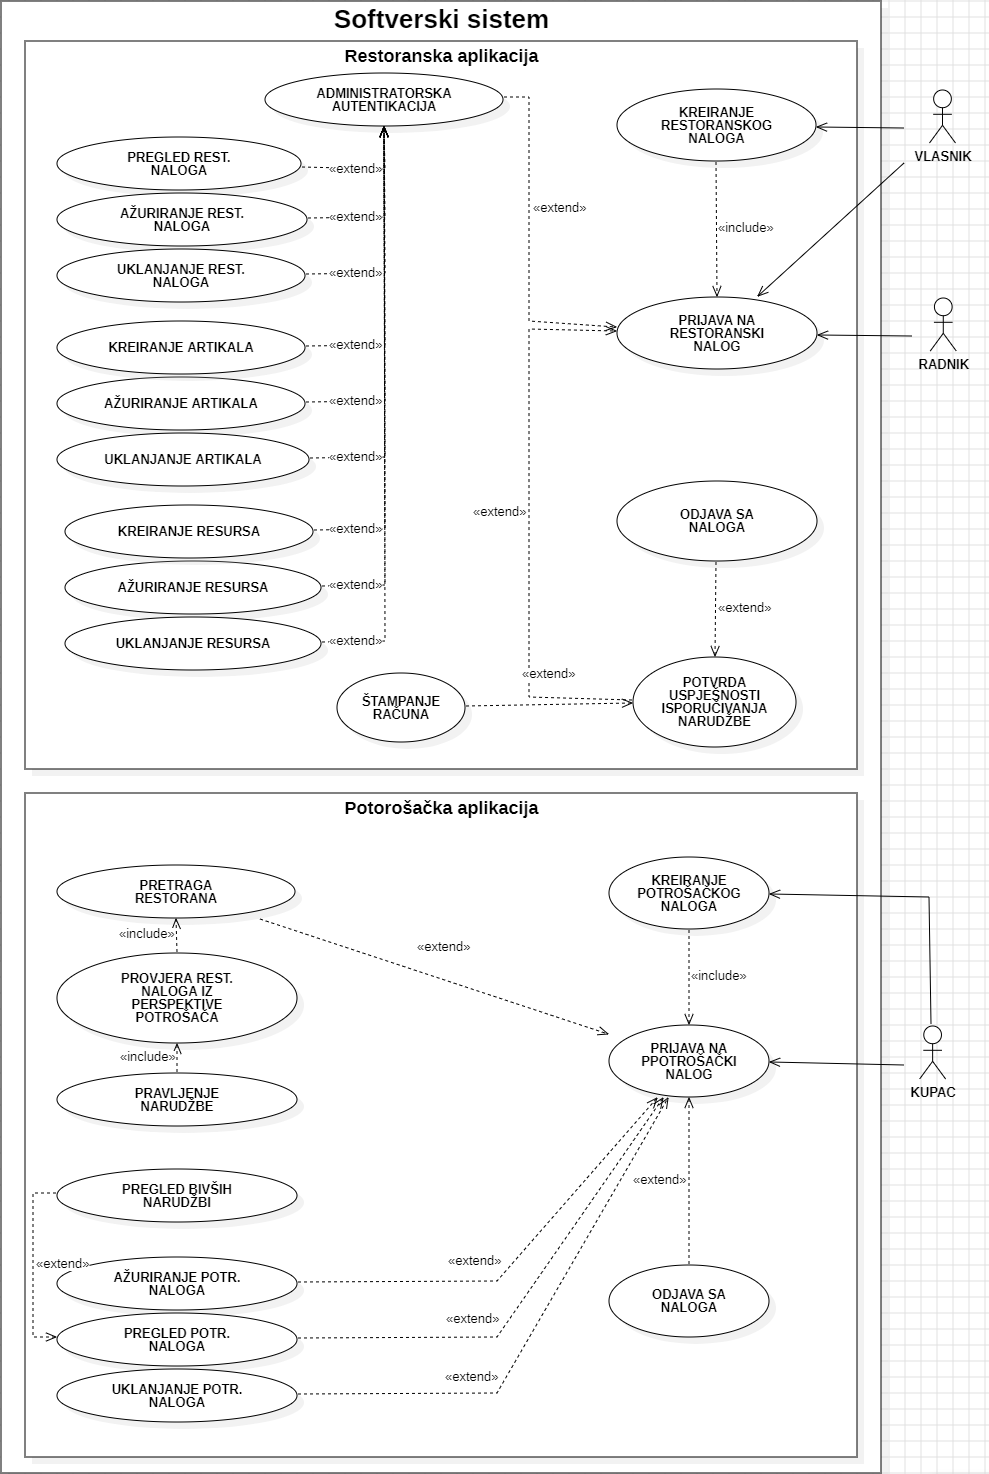
\includegraphics[width=14.5cm]{./img/zahtjevi_sistema.png}
\end{center}

Funkcionalnostima iz dijagrama se dodaju sljedeće oznake:

\begin{center}
	\begin{tabular}{|l|l|}
		\hline
		\textbf{Oznaka} & \textbf{Funkcionalnost} \\ \hline
		\hline
		F1  & KREIRANJE REST. NALOGA \\ \hline
		F2  & PRIJAVA NA RESTORANSKI NALOG \\ \hline
		F3  & ADMINISTRATORSKA AUTENTIKACIJA \\ \hline
		F4  & PREGLED REST. NALOGA IZ PERSPEKTIVE VLASNIKA \\ \hline
		F5  & AŽURIRANJE REST. NALOGA \\ \hline
		F6  & UKLANJANJE REST. NALOGA \\ \hline
		F7  & KREIRANJE ARTIKLA \\ \hline
		F8  & AŽURIRANJE ARTIKLA \\ \hline
		F9  & UKLANJANJE ARTIKLA \\ \hline
		F10 & KREIRANJE RESURSA \\ \hline
		F11 & AŽURIRANJE RESURSA \\ \hline
		F12 & UKLANJANJE RESURSA \\ \hline
		F13 & POTVRDA USPJEŠNOSTI ISPORUČIVANJA NARUDŽBE \\ \hline
		F14 & KREIRANJE POTROŠAČKOG NALOGA \\ \hline
		F15 & PRIJAVA NA POTROŠAČKI NALOG \\ \hline
		F16 & PRETRAGA RESTORANA \\ \hline
		F17 & PREGLED REST. NALOGA IZ PERSPEKTIVE POTROŠAČA \\ \hline
		F18 & PRAVLJENJE NARUDŽBE \\ \hline
		F19 & AŽURIRANJE POTROŠAČKOG NALOGA \\ \hline
		F20 & PREGLED POTROŠAČKOG NALOGA \\ \hline
		F21 & PREGLED BIVŠIH NARUDŽBI \\ \hline
		F22 & UKLANJANJE POTROŠAČKOG NALOGA \\ \hline
		F23 & ODJAVA SA NALOGA \\ \hline
		F24 & ŠTAMPANJE RAČUNA \\ \hline
		F25 & POVRATAK NA PRETHODNI PROZOR \\ \hline % TODO: dijagram

	\end{tabular}
\end{center}

\section{Klase korisnika i njihove karakteristike}
Klase korisnika su ranije navedeni:

\begin{enumerate}
	\itemsep0em
	\item \textbf{Kupci},\\
		koji će imati pristup potrošačkoj aplikaciji, te sa njom moći
		da kreiraju, uklanjaju i održavaju svoj nalog, te da
		nađu željeni restoran i prave narudžbu u njemu.
	\item \textbf{Vlasnici},\\
		koji će imati pristup restoranskoj aplikaciji, te sa njom,
		uz odgovarajući administratorski pristup, moći
		da kreiraju, uklanjaju i održavaju nalog restorana,
		da kreiraju, uklanjaju i održavaju resurse restorana,
		da kreiraju, uklanjaju i održavaju artikle restorana
		i da otpisuju isporučene narudžbe.
	\item \textbf{Radnici},\\
		koji će imati pristup restoranskoj aplikaciji, te sa njom moći
		da se prijave na nalog restorana,
		i da otpisuju isporučene narudžbe.
\end{enumerate}

\section{Radno okruženje}
Softverski sistem je predviđen da funkcioniše na "desktop" računarima
na operativnom sistemu Windows.

\section{Eksterni interfejsi}

\subsection{Korisnički interfejsi}

Korisnički interfejs je dat u obliku grafičkih komponenti napravljenih pomoću
grafičke biblioteke WinForms. Te komponente su:

\begin{enumerate}
	\itemsep0em
	\item Komponenta za prijavu na nalog
	\item Komponenta za odjavu sa naloga
	\item Komponenta za administratorsku autentikaciju
	\item Komponenta za kreiranje (naloga, artikala i resursa)
	\item Komponenta za ažuriranje (naloga, artikala i resursa)
	\item Komponenta za uklanjanje (naloga, artikala i resursa)
	\item Komponenta za pretragu restorana
	\item Komponenta za pravljenje narudžbe
	\item Komponenta za potvrdu željene radnje
\end{enumerate}

\subsection{Hardverski interfejsi}

Hardverski zahtjevi softverskog sistema su trivijalni.
Softverski sistem će funkcionisati na bilo kom hardverskom sistemu
koji može da podnese grafičke prozore kreirane pomoću biblioteke WinForms.
Takav sistem aproksimativno uključuje:

\begin{itemize}
	\itemsep0em
	\item CPU: x86 ili x64, 1GHz ili više
	\item RAM: 512 MB ili više, 1600MHz ili više
	\item HDD: 4.5GB ili više
\end{itemize}

Ovakav hardverski sistem uzima u obzir obe aplikacije softverskog sistema.
Naknadno, hardverski sistem koji podržava restoransku aplikaciju uključuje
aparat za štampanje računa i, izborno, ekran osjetljiv na dodir.

\subsection{Softverski interfejsi}

Pored operativnog sitema Windows i
biblioteka koje su svakako uključene u sam sistem,
softverski sistem nije zavisan od nekog drugog softvera.

\subsection{Komunikacioni interfejsi}

Ova verzija softverskog sistema
ne pravi nikakve spoljašnje veze putem mreže
(Internet, LAN, itd).
Sistem komunicira korištenjem lokalnih datoteka,
kojim mogu pristupiti sve instance softverskog sistema
koje rade nad istom čvrstom memorijom.

% \section{Korisnička dokumentacija}

\newgeometry{top=1cm,left=3cm,bottom=0.1cm}

\chapter{Zahtjevi sistema}

\begin{center}
\begin{tabular}{|l|l|}
	\hline
	Oznaka: & F1 \\
	\hline
	Naziv: & KREIRANJE RESTORANSKOG NALOGA \\
	\hline
	\smash{\raisebox{0ex}{Kratak opis:}} & Funkcionalnost koja vlasnicima omogućava\\
	&kreiranje naloga za svoj restoran \\
	\hline
	Učesnici: & Vlasnik \\
	\hline
	Preduslovi: & Vlasnik ima rest. aplikaciju na svome računaru \\
	\hline
	\smash{\raisebox{0ex}{Tok akcija:}}
	& 1. Vlasnik klikne na dugme "KREIRANJE\\
	& \hspace{10pt} NALOGA" \\
	& 2. Vlasnik unosi tražene podatke \\
	& 3. Vlasnik klikne na dugme "DALJE" \\
	\hline
	\smash{\raisebox{0ex}{Postuslovi:}}
	& Nalog se pohranjuje u bazi podataka. Vlasnik \\
	& je obaviješten o uspješnosti kreiranja naloga.\\
	& Vlasnik je preusmjeren na prozor za prijavu \\
	& na nalog. \\
	\hline
	\smash{\raisebox{0ex}{Alternativni tokovi i izuzeci:}}

	& 3.a. Nalog sa datim podacima već postoji \\
	& Postuslov: Vlasnik je obaviješten o neuspješnosti \\
	& \hspace{51pt} kreiranja naloga. \\

	&\\

	& 3.b. Uneseni podaci nisu ispravni \\
	& Postuslov: Vlasnik je obaviješten o neuspješnosti \\
	& \hspace{51pt} kreiranja naloga. \\

	\hline

\end{tabular}
\end{center}

\begin{center}
	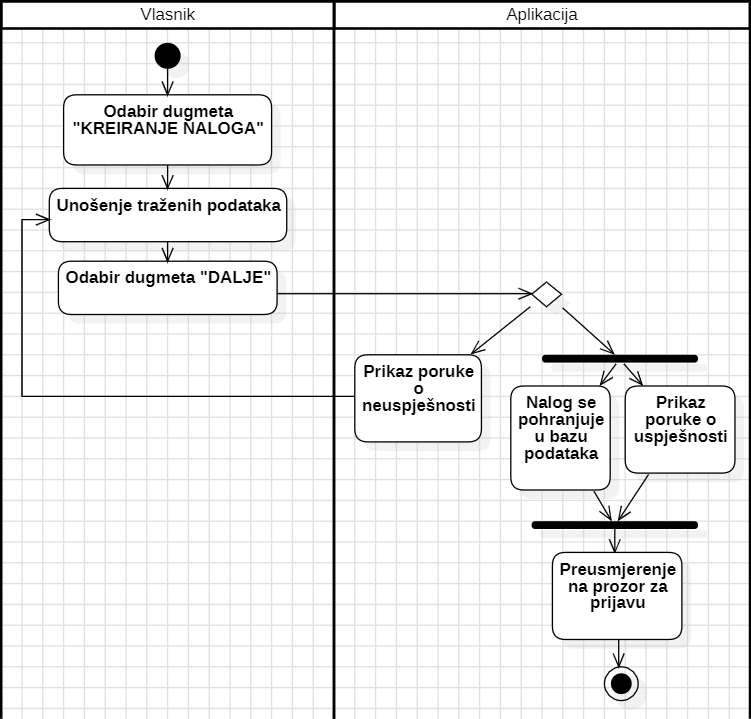
\includegraphics[width=12cm]{./img/01.png}
\end{center}

\begin{center}
\begin{tabular}{|l|l|}
	\hline
	Oznaka: & F2 \\
	\hline
	Naziv: & PRIJAVA NA RESTORANSKI NALOG \\
	\hline
	\smash{\raisebox{0ex}{Kratak opis:}}
	& Funkcionalnost koja vlasniku ili radniku\\
	& daje pristup restoranskom nalogu \\
	\hline
	Učesnici: & Vlasnik ili radnik, ispod naveden kao korisnik \\
	\hline
	Preduslovi: & Vlasnik ima odgovarajući nalog za svoj restoran.\\
	& Korisnik ima rest. aplikaciju na svom računaru. \\
	\hline
	\smash{\raisebox{0ex}{Tok akcija:}}
	& 1. Korisnik klikne na dugme "PRIJAVA NA\\
	& \hspace{10pt} NALOG" \\
	& 2. Korisnik unosi korisničko ime i šifru \\
	& 3. Korisnik klikne na dugme "DALJE" \\
	\hline
	\smash{\raisebox{0ex}{Postuslovi:}}
	& Korisnik je preusmjeren na prozor koji mu\\
	& omogućava da pristupi narudžbama i \\
	& adminisratorskim opcijama. \\
	\hline
	\smash{\raisebox{0ex}{Alternativni tokovi i izuzeci:}}

	& 3.a. Uneseni podaci ne odgovaraju nekom nalogu \\
	& Postuslov: Korisnik je obaviješten o neuspješnom\\
	& \hspace{50pt} pokušaju pristupa \\

	&\\

	& 3.b. Uneseni podaci nisu ispravni \\
	& Postuslov: Korisnik je obaviješten o neuspješnom\\
	& \hspace{50pt} pokušaju pristupa \\

	\hline

\end{tabular}
\end{center}

\begin{center}
	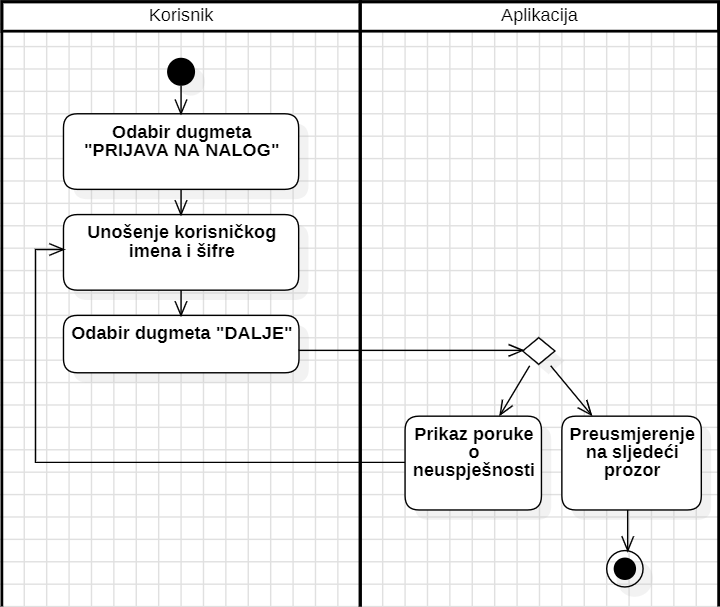
\includegraphics[width=12cm]{./img/02.png}
\end{center}

\pagebreak

\begin{center}
\begin{tabular}{|l|l|}
	\hline
	Oznaka: & F3 \\
	\hline
	Naziv: & ADMINISTRATORSKA AUTENTIKACIJA \\
	\hline
	\smash{\raisebox{0ex}{Kratak opis:}}
	& Funkcionalnost koja vlasnicima omogućava\\
	& pravo kreiranja, pregleda i ažuriranja \\
	& podataka kojima radnici nemaju pristup. \\
	\hline
	Učesnici: & Vlasnik \\
	\hline
	Preduslovi: & Vlasnik ima odgovarajući nalog za svoj restoran.\\
	& Vlasnik je prijavljen na svoj restoranski nalog. \\
	\hline
	\smash{\raisebox{0ex}{Tok akcija:}}
	& 1. Vlasnik klikne na dugme\\
	& \hspace{10pt} "ADMINISTRATORSKA AUTENTIKACIJA" \\
	& 2. Vlasnik unosi administratorsku šifru \\
	& 3. Vlasnik klikne na dugme "DALJE" \\
	\hline

	\smash{\raisebox{0ex}{Postuslovi:}}
	& Vlasnik je preusmjeren na administratorski prozor. \\
	\hline
	\smash{\raisebox{0ex}{Alternativni tokovi i izuzeci:}}

	& 3.a. Uneseni podatak nije ispravan \\
	& Postuslov: Vlasnik je obaviješten o neuspješnom\\
	& \hspace{50pt} pokušaju pristupa. \\

	\hline

\end{tabular}
\end{center}

\begin{center}
	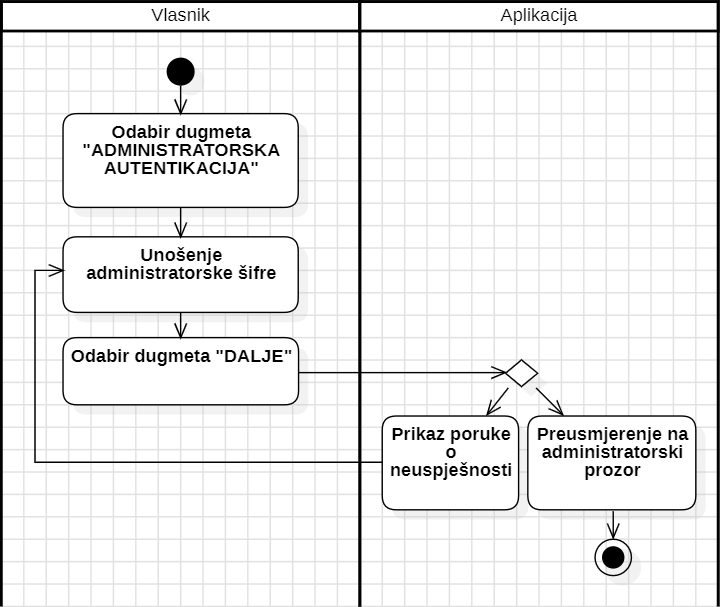
\includegraphics[width=14cm]{./img/03.png}
\end{center}

\pagebreak

\begin{center}
\begin{tabular}{|l|l|}
	\hline
	Oznaka: & F4 \\
	\hline
	Naziv: & PREGLED RESTORANSKOG NALOGA IZ \\
	& PERSPEKTIVE VLASNIKA \\
	\hline
	\smash{\raisebox{0ex}{Kratak opis:}}
	& Funkcionalnost koja vlasnicima omogućava\\
	& pregled naloga i statističkih podataka svog \\
	& restorana \\
	\hline
	Učesnici: & Vlasnik \\
	\hline
	Preduslovi: & Vlasnik ima odgovarajući nalog za svoj restoran.\\
	& Vlasnik je prijavljen na svoj restoranski nalog. \\
	& Vlasnik ima administratorsku pristup. \\
	\hline
	\smash{\raisebox{0ex}{Tok akcija:}}
	& 1. Vlasnik klikne na dugme \\
	& \hspace{10pt}"PREGLEDAJ NALOG" \\
	\hline
	\smash{\raisebox{0ex}{Postuslovi:}}
	& Vlasnik je preusmjeren na prozor na kojem\\
	& može da vidi svoj nalog. \\
	\hline
	\smash{\raisebox{0ex}{Alternativni tokovi i izuzeci:}}
	& Nema. \\
	\hline

\end{tabular}
\end{center}

\begin{center}
	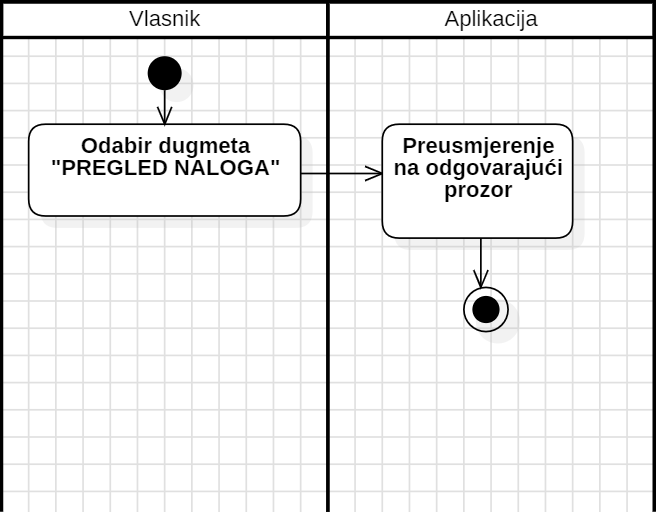
\includegraphics[width=14cm]{./img/04.png}
\end{center}

\pagebreak

\begin{center}
\begin{tabular}{|l|l|}
	\hline
	Oznaka: & F5 \\
	\hline
	Naziv: & AŽURIRANJE RESTORANSKOG NALOGA \\
	\hline
	\smash{\raisebox{0ex}{Kratak opis:}}
	& Funkcionalnost koja vlasnicima omogućava\\
	& ažuriranje podataka o nalogu svog restorana.\\
	\hline
	Učesnici: & Vlasnik \\
	\hline
	Preduslovi: & Vlasnik ima odgovarajući nalog za svoj restoran.\\
	& Vlasnik je prijavljen na svoj restoranski nalog. \\
	& Vlasnik ima administratorski pristup. \\
	\hline
	\smash{\raisebox{0ex}{Tok akcija:}}
	& 1. Vlasnik klikne na dugme "AŽURIRAJ NALOG" \\
	& 2. Vlasnik napravi željene izmjene \\
	& 3. Vlasnik klikne na dugme "POTVRDI" \\
	\hline
	\smash{\raisebox{0ex}{Postuslovi:}}
	& U bazi podataka se dešavaju tražene izmejene. \\
	& Vlasnik je vraćen na prethodni prozor. \\
	\hline
	\smash{\raisebox{0ex}{Alternativni tokovi i izuzeci:}}

	& 3.a. Uneseni podaci nisu ispravni \\
	& Postuslov: Vlasnik je obaviješten o neuspješnom \\
	& \hspace{51pt} pokušaju izmjene. \\

	\hline

\end{tabular}
\end{center}

\begin{center}
	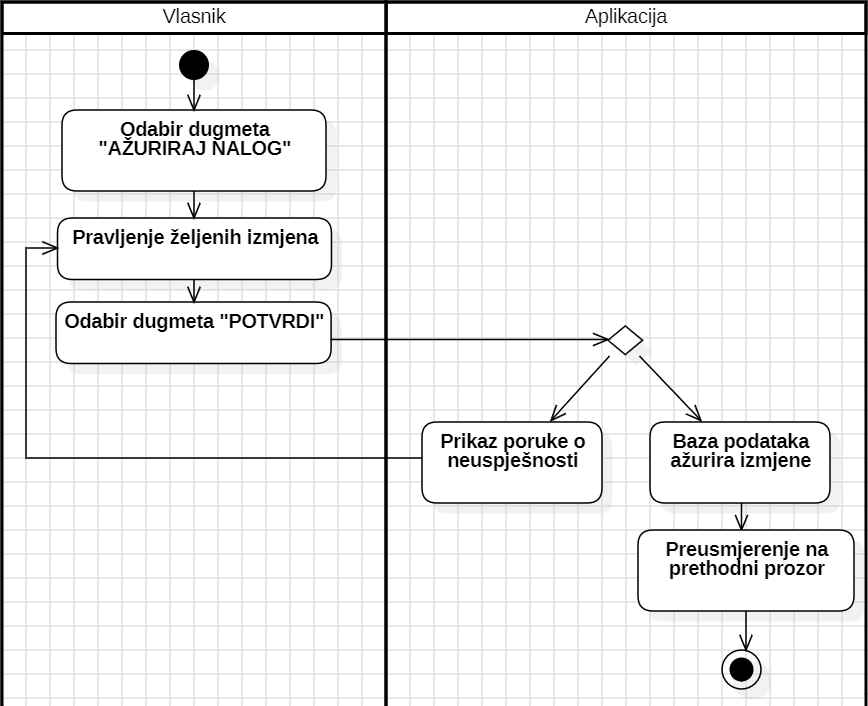
\includegraphics[width=14cm]{./img/05.png}
\end{center}

\pagebreak

\begin{center}
\begin{tabular}{|l|l|}
	\hline
	Oznaka: & F6 \\
	\hline
	Naziv: & UKLANJANJE RESTORANSKOG NALOGA \\
	\hline
	\smash{\raisebox{0ex}{Kratak opis:}}
	& Funkcionalnost koja vlasnicima omogućava \\
	& uklanjanje svog rest. naloga iz baze podataka \\
	\hline
	Učesnici: & Vlasnik \\
	\hline
	Preduslovi:
	& Vlasnik ima odgovarajući nalog za svoj restoran. \\
	& Vlasnik je prijavljen na svoj restoranski nalog. \\
	& Vlasnik ima administratorski pristup. \\
	\hline
	\smash{\raisebox{0ex}{Tok akcija:}}
	& 1. Vlasnik klikne na dugme "UKLONI NALOG" \\
	& 2. Vlasnik je preusmjeren na prozor na \\
	& \hspace{10pt} kojem se nalazi tekstualno polje na kojem \\
	& \hspace{10pt} piše "Da li ste sigurni da želite da uklonite\\
	& \hspace{10pt} svoj nalog?" i dugmad "DA" i "NE". \\
	& 3. Vlasnik klikne na "DA". \\
	\hline
	\smash{\raisebox{0ex}{Postuslovi:}}
	& Nalog se uklanja, i vlasnik se vraća na \\
	& \textit{početni prozor} rest. aplikacije. \\
	\hline
	\smash{\raisebox{0ex}{Alternativni tokovi i izuzeci:}}

	& 3.a. Vlasnik klikne na dugme "NE" \\
	& Postuslov: Vlasnik se vraća na prethodni \\
	& \hspace{50pt} prozor restoranske aplikacije. \\

	&\\

	& 3.b. Vlasnik klikne na dugme "DA", nije \\
	& \hspace{21pt} moguće ukloniti nalog \\
	& Postuslov: Vlasnik je obaviješten o neuspješnosti \\
	& \hspace{51pt} uklanjanja naloga. Vlasnik je vraćen \\
	& \hspace{51pt} na prethodni prozor. \\

	\hline

\end{tabular}
\end{center}

\begin{center}
	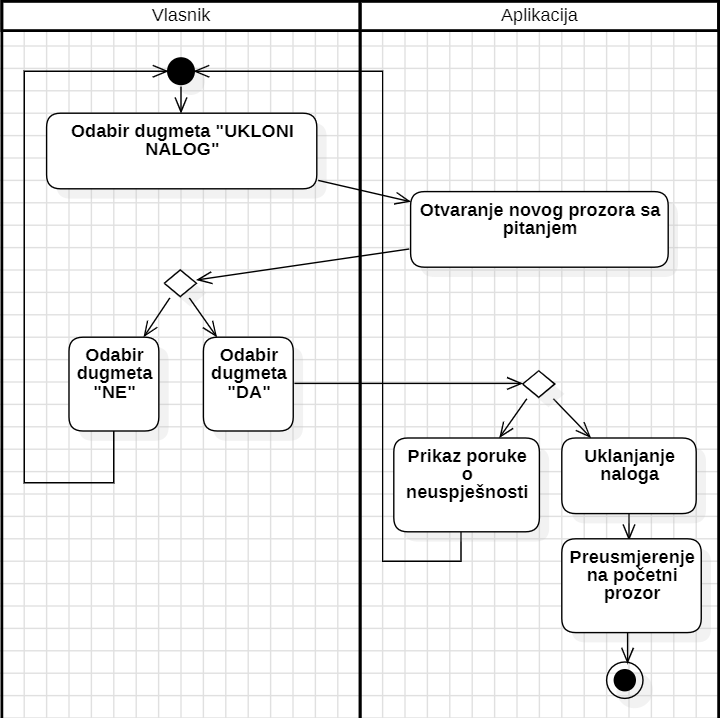
\includegraphics[width=14cm]{./img/06.png}
\end{center}

\pagebreak

\begin{center}
\begin{tabular}{|l|l|}
	\hline
	Oznaka: & F7 \\
	\hline
	Naziv: & KREIRANJE ARTIKLA \\
	\hline
	\smash{\raisebox{0ex}{Kratak opis:}}
	& Funkcionalnost koja vlasnicima omogućava\\
	& kreiranje novih artikala u ponudi restorana \\
	\hline
	Učesnici: & Vlasnik \\
	\hline
	Preduslovi:
	& Vlasnik ima odgovarajući nalog za svoj restoran. \\
	& Vlasnik je prijavljen na svoj restoranski nalog. \\
	& Vlasnik ima administratorski pristup. \\
	\hline
	\smash{\raisebox{0ex}{Tok akcija:}}
	& 1. Vlasnik klikne na dugme "KREIRAJ ARTIKL" \\
	& 2. Vlasnik unosi tražene podatke \\
	& 3. Vlasnik klikne na dugme "DALJE" \\
	\hline
	\smash{\raisebox{0ex}{Postuslovi:}}
	& Artikl se pohranjuje u bazi podataka. Vlasnik \\
	& je obaviješten o uspješnosti kreiranja artikla.\\
	& Vlasnik je vraćen na prethodni prozor. \\
	\hline
	\smash{\raisebox{0ex}{Alternativni tokovi i izuzeci:}}

	& 3.a. Uneseni podaci nisu ispravni \\
	& Postuslov: Vlasnik je obaviješten o neuspješnosti \\
	& \hspace{51pt} kreiranja artikla. \\

	\hline

\end{tabular}
\end{center}

\begin{center}
	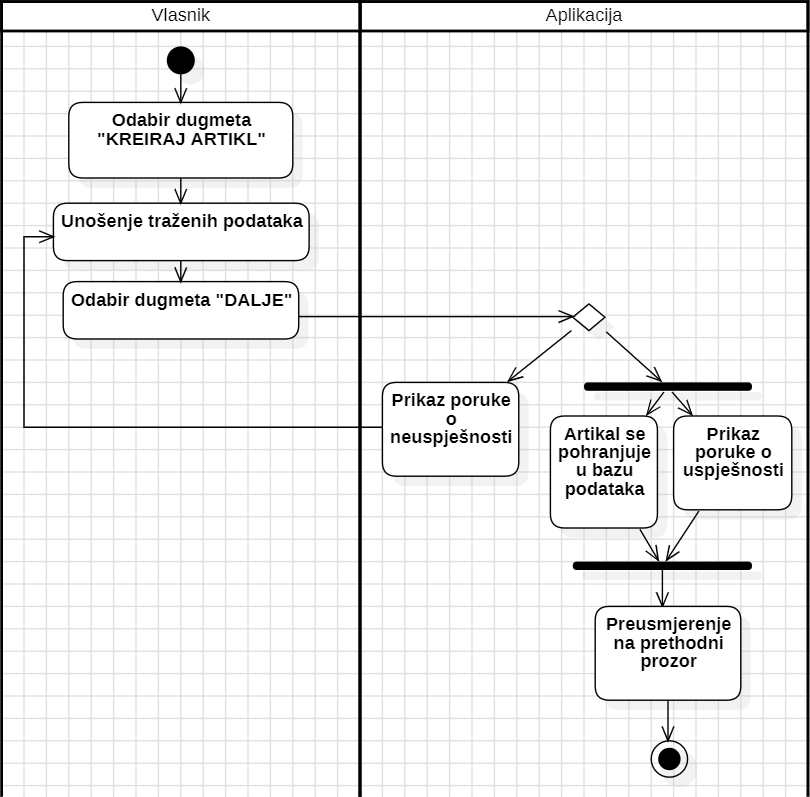
\includegraphics[width=14cm]{./img/07.png}
\end{center}

\pagebreak

\begin{center}
\begin{tabular}{|l|l|}
	\hline
	Oznaka: & F8 \\
	\hline
	Naziv: & AŽURIRANJE ARTIKLA \\
	\hline
	\smash{\raisebox{0ex}{Kratak opis:}}
	& Funkcionalnost koja vlasnicima omogućava\\
	& ažuriranje postojećih artikala u ponudi restorana \\
	\hline
	Učesnici: & Vlasnik \\
	\hline
	Preduslovi:
	& Vlasnik ima odgovarajući nalog za svoj restoran. \\
	& Vlasnik je prijavljen na svoj restoranski nalog. \\
	& Vlasnik ima administratorski pristup. \\
	\hline
	\smash{\raisebox{0ex}{Tok akcija:}}
	& 1. Vlasnik klikne na dugme "AŽURIRAJ ARTIKL" \\
	& 2. Vlasnik bira koji artikl ažurira \\
	& 3. Vlasnik ažurira željene podatke \\
	& 4. Vlasnik klikne na dugme "POTVRDI" \\
	\hline
	\smash{\raisebox{0ex}{Postuslovi:}}
	& Ažurira se baza podataka. Vlasnik \\
	& je obaviješten o uspješnosti ažuriranja artikla.\\
	& Vlasnik se vraća na prethodni prozor.\\
	\hline
	\smash{\raisebox{0ex}{Alternativni tokovi i izuzeci:}}

	& 4.a. Uneseni podaci nisu ispravni \\
	& Postuslov: Vlasnik je obaviješten o neuspješnosti \\
	& \hspace{51pt} ažuriranja artikla. \\

	\hline

\end{tabular}
\end{center}

\begin{center}
	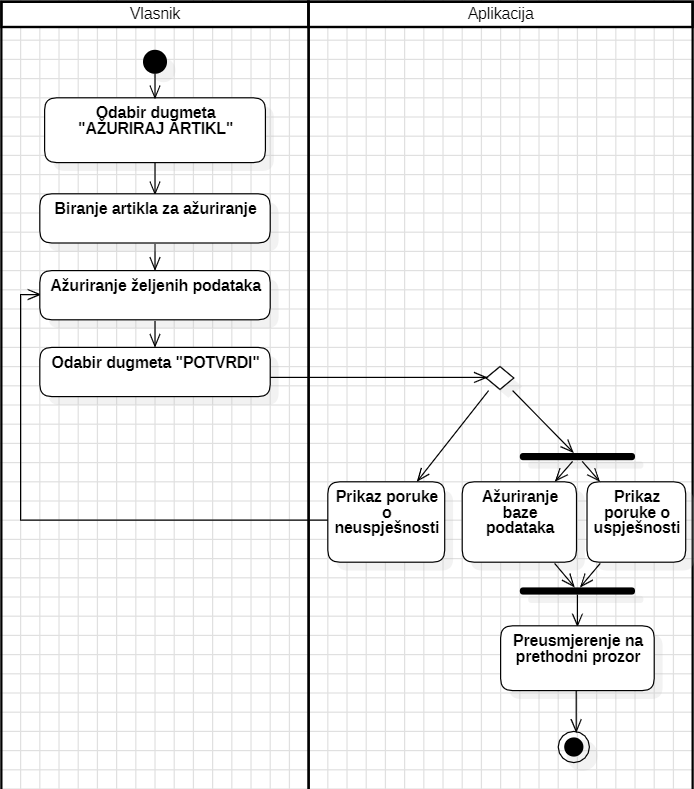
\includegraphics[width=14cm]{./img/08.png}
\end{center}

\pagebreak

\begin{center}
\begin{tabular}{|l|l|}
	\hline
	Oznaka: & F9 \\
	\hline
	Naziv: & UKLANJANJE ARTIKLA \\
	\hline
	\smash{\raisebox{0ex}{Kratak opis:}}
	& Funkcionalnost koja vlasnicima omogućava\\
	& uklanjanje postojećih artikala iz ponude restorana \\
	\hline
	Učesnici: & Vlasnik \\
	\hline
	Preduslovi:
	& Vlasnik ima odgovarajući nalog za svoj restoran. \\
	& Vlasnik je prijavljen na svoj restoranski nalog. \\
	& Vlasnik ima administratorski pristup. \\
	\hline
	\smash{\raisebox{0ex}{Tok akcija:}}
	& 1. Vlasnik klikne na dugme "UKLONI ARTIKL" \\
	& 2. Vlasnik bira koji artikl uklanja\\
	& 3. Vlasnik klikne na dugme "UKLONI" \\
	& 4. Vlasnik je preusmjeren na prozor na \\
	& \hspace{10pt} kojem se nalazi tekstualno polje na kojem \\
	& \hspace{10pt} piše "Da li ste sigurni da želite da uklonite\\
	& \hspace{10pt} artikl?" i dugmad "DA" i "NE" \\
	& 5. Vlasnik klikne na "DA" \\
	\hline
	\smash{\raisebox{0ex}{Postuslovi:}}
	& Artikl se uklanja iz baze podataka. Vlasnik \\
	& je obaviješten o uspješnosti uklanjanja artikla.\\
	& Vlasnik se vraća na administrativni prozor. \\
	\hline
	\smash{\raisebox{0ex}{Alternativni tokovi i izuzeci:}}

	& 5.a. Vlasnik klikne na dugme "NE" \\
	& Postuslov: Vlasnik se vraća na prethodni \\
	& \hspace{50pt} prozor restoranske aplikacije. \\

	&\\

	& 5.b. Vlasnik klikne na dugme "DA", nije \\
	& \hspace{21pt} moguće ukloniti nalog \\
	& Postuslov: Vlasnik je obaviješten o neuspješnosti \\
	& \hspace{51pt} uklanjanja naloga. Vlasnik je vraćen \\
	& \hspace{51pt} na administrativni prozor. \\

	\hline

\end{tabular}
\end{center}

\begin{center}
	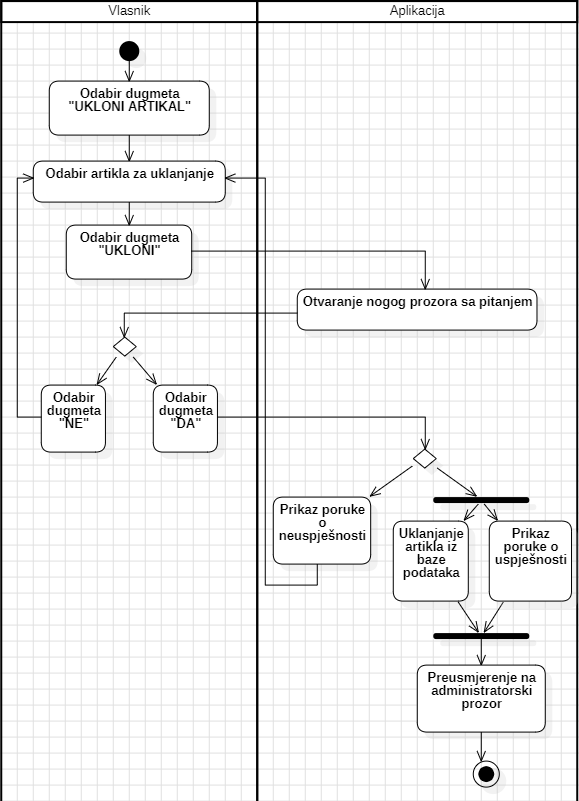
\includegraphics[width=14cm]{./img/09.png}
\end{center}

\pagebreak

\begin{center}
\begin{tabular}{|l|l|}
	\hline
	Oznaka: & F10 \\
	\hline
	Naziv: & KREIRANJE RESURSA \\
	\hline
	\smash{\raisebox{0ex}{Kratak opis:}}
	& Funkcionalnost koja vlasnicima omogućava \\
	& definisanje novog resursa koji će biti u inventaru \\
	& restorana. \\
	\hline
	Učesnici: & Vlasnik \\
	\hline
	Preduslovi:
	& Vlasnik ima odgovarajući nalog za svoj restoran. \\
	& Vlasnik je prijavljen na svoj restoranski nalog. \\
	& Vlasnik ima administratorski pristup. \\
	\hline
	\smash{\raisebox{0ex}{Tok akcija:}}
	& 1. Vlasnik klikne na dugme "KREIRAJ RESURS" \\
	& 2. Vlasnik unosi tražene podatke \\
	& 3. Vlasnik klikne na dugme "DALJE" \\
	\hline
	\smash{\raisebox{0ex}{Postuslovi:}}
	& Resurs se pohranjuje u bazi podataka. Vlasnik \\
	& je obaviješten o uspješnosti definisanja novog \\
	& resursa. Vlasnik se vraća na administrativni prozor. \\
	\hline
	\smash{\raisebox{0ex}{Alternativni tokovi i izuzeci:}}

	& 3.a. Resurs već postoji \\
	& Postuslov: Vlasnik je obaviješten o neuspješnosti \\
	& \hspace{51pt} definisanja novog resursa. \\

	\hline

\end{tabular}
\end{center}

\begin{center}
	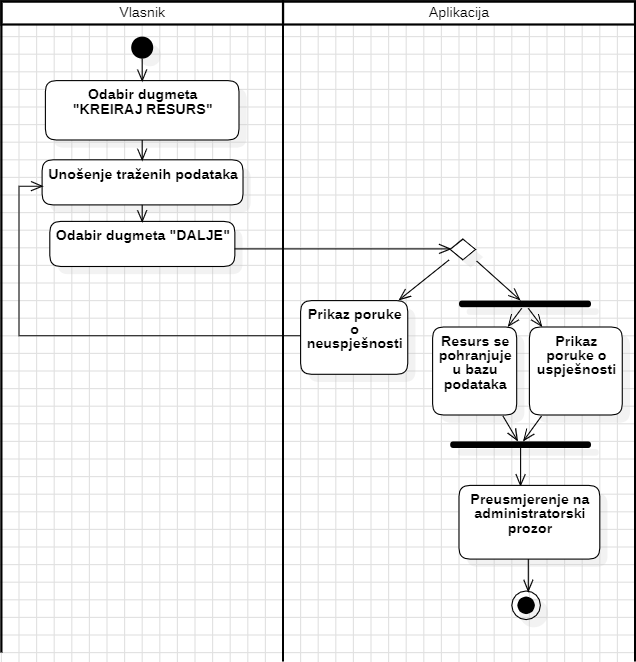
\includegraphics[width=14cm]{./img/10.png}
\end{center}

\pagebreak

\begin{center}
\begin{tabular}{|l|l|}
	\hline
	Oznaka: & F11 \\
	\hline
	Naziv: & AŽURIRANJE RESURSA \\
	\hline
	\smash{\raisebox{0ex}{Kratak opis:}}
	& Funkcionalnost koja vlasnicima omogućava\\
	& ažuriranje resursa restorana. \\
	\hline
	Učesnici: & Vlasnik \\
	\hline
	Preduslovi:
	& Vlasnik ima odgovarajući nalog za svoj restoran. \\
	& Vlasnik je prijavljen na svoj restoranski nalog. \\
	& Vlasnik ima administratorski pristup. \\
	\hline
	\smash{\raisebox{0ex}{Tok akcija:}}
	& 1. Vlasnik klikne na dugme "AŽURIRAJ RESURS" \\
	& 2. Vlasnik bira koji resurs ažurira \\
	& 3. Vlasnik ažurira željene podatke \\
	& 4. Vlasnik klikne na dugme "POTVRDI" \\
	\hline
	\smash{\raisebox{0ex}{Postuslovi:}}
	& Ažurira se baza podataka. Vlasnik \\
	& je obaviješten o uspješnosti ažuriranja resursa. \\
	& Vlasnik se vraća na administratorski prozor. \\
	\hline
	\smash{\raisebox{0ex}{Alternativni tokovi i izuzeci:}}

	& 4.a. Uneseni podaci nisu ispravni \\
	& Postuslov: Vlasnik je obaviješten o neuspješnosti \\
	& \hspace{51pt} ažuriranja resursa. \\

	\hline

\end{tabular}
\end{center}

\begin{center}
	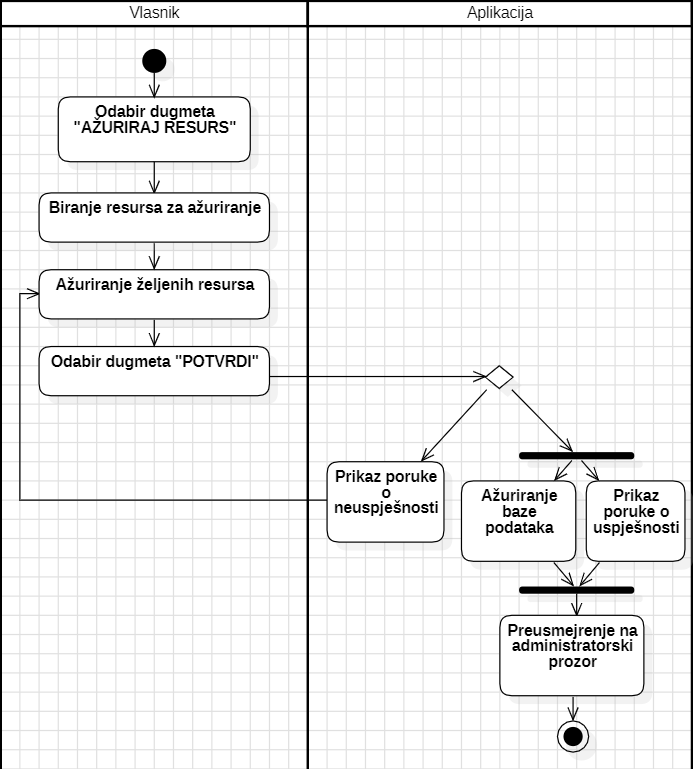
\includegraphics[width=14cm]{./img/11.png}
\end{center}

\pagebreak

\begin{center}
\begin{tabular}{|l|l|}
	\hline
	Oznaka: & F12 \\
	\hline
	Naziv: & UKLANJANJE RESURSA \\
	\hline
	\smash{\raisebox{0ex}{Kratak opis:}}
	& Funkcionalnost koja vlasnicima omogućava\\
	& uklanjanje resursa iz inventara restorana \\
	\hline
	Učesnici: & Vlasnik \\
	\hline
	Preduslovi:
	& Vlasnik ima odgovarajući nalog za svoj restoran. \\
	& Vlasnik je prijavljen na svoj restoranski nalog. \\
	& Vlasnik ima administratorski pristup. \\
	\hline
	\smash{\raisebox{0ex}{Tok akcija:}}
	& 1. Vlasnik klikne na dugme "UKLONI RESURS" \\
	& 2. Vlasnik bira koji resurs uklanja \\
	& 3. Vlasnik klikne na dugme "UKLONI" \\
	& 4. Vlasnik je preusmjeren na prozor na \\
	& \hspace{10pt} kojem se nalazi tekstualno polje na kojem \\
	& \hspace{10pt} piše "Da li ste sigurni da želite da uklonite \\
	& \hspace{10pt} resurs?" i dugmad "DA" i "NE" \\
	& 5. Vlasnik klikne na ”DA” \\
	\hline
	\smash{\raisebox{0ex}{Postuslovi:}}
	& Resurs se uklanja iz baze podataka. Vlasnik \\
	& je obaviješten o uspješnosti uklanjanja resursa.\\
	& Vlasnik se vraća na administrativni prozor. \\
	\hline
	\smash{\raisebox{0ex}{Alternativni tokovi i izuzeci:}}

	& 5.a. Vlasnik klikne na dugme "NE" \\
	& Postuslov: Vlasnik se vraća na prethodni \\
	& \hspace{50pt} prozor restoranske aplikacije. \\

	&\\

	& 5.b. Vlasnik klikne na dugme "DA", nije \\
	& \hspace{21pt} moguće ukloniti resurs \\
	& Postuslov: Vlasnik je obaviješten o neuspješnosti \\
	& \hspace{51pt} uklanjanja resursa. Vlasnik je vraćen \\
	& \hspace{51pt} na prethodni prozor. \\

	\hline

\end{tabular}
\end{center}

\begin{center}
	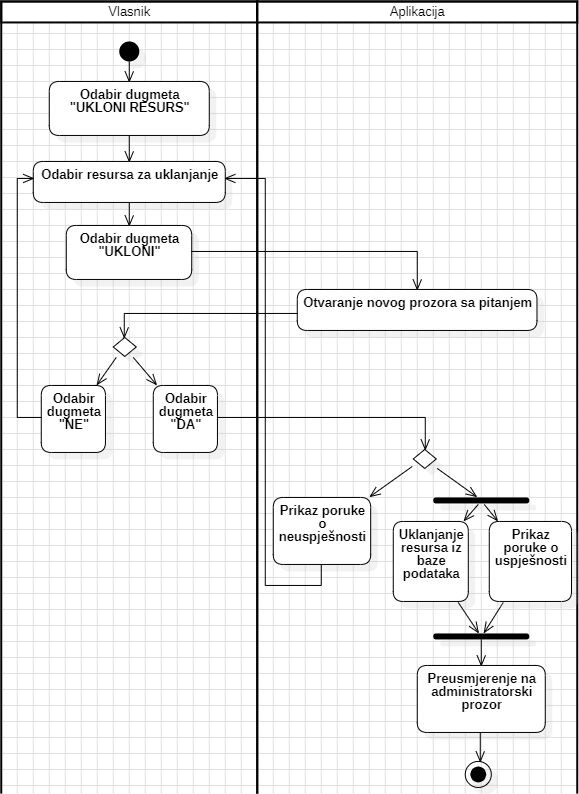
\includegraphics[width=14cm]{./img/12.png}
\end{center}

\pagebreak

% TODO: Upozori kada je resurs pri kraju

\begin{center}
\begin{tabular}{|l|l|}
	\hline
	Oznaka: & F13 \\
	\hline
	\smash{\raisebox{0ex}{Naziv:}}
	& POTVRDA USPJEŠNOSTI ISPORUČIVANJA \\
	& NARUDŽBE \\
	\hline
	\smash{\raisebox{0ex}{Kratak opis:}}
	& Funkcionalnost koja vlasnicima i radnicima \\
	& omogućava da potvrde da je narudžba napravljena \\
	&i isporučena \\
	\hline
	Učesnici: & Vlasnik ili radnik, ispod naveden kao korisnik \\
	\hline
	Preduslovi:
	& Korisnik ima rest. aplikaciju na svome računaru. \\
	& Korisnik je prijavljen na nalog restorana.  \\
	& Korisnik je na prozoru koji je odstpan odmah nakon\\&prijave. \\
	\hline
	\smash{\raisebox{0ex}{Tok akcija:}}
	& 1. Korisnik klikne na dugme "POGLEDAJ \\& \hspace{10pt} NARUDŽBE" \\
	& 2. Korisnik klikne na dugme pored narudžbe koja\\&je isporučena\\
	& 3. Korisnik ponavlja korak 2 \\
	\hline
	\smash{\raisebox{0ex}{Postuslovi:}}
	& Narudžba asocirana sa dugmetom koje je korisnik\\
	& kliknuo se uklanjanja s reda narudžbi. \\
	\hline
	\smash{\raisebox{0ex}{Alternativni tokovi i izuzeci:}}

	& 2.a. Kritično mala količina resursa \\
	& Postuslov: Korisnik je obaviješten da je neophodno\\
	& \hspace{50pt} dodati još resursa. \\

	\hline

\end{tabular}
\end{center}

\begin{center}
	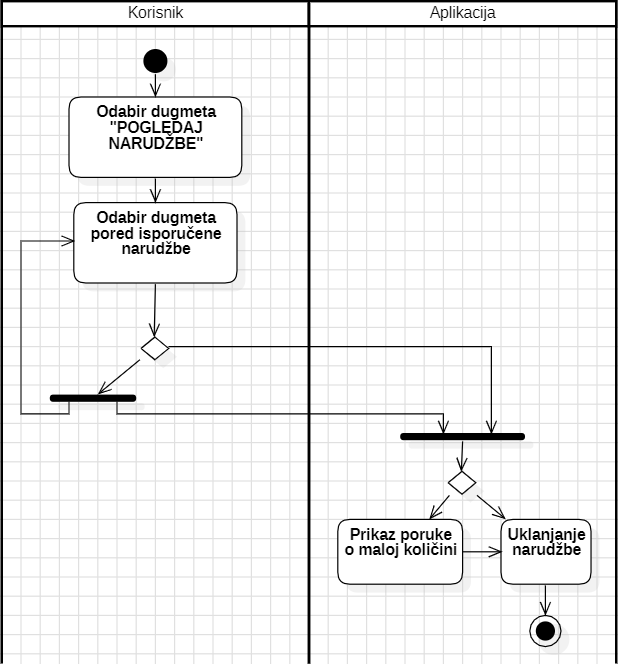
\includegraphics[width=14cm]{./img/13.png}
\end{center}

\pagebreak

\begin{center}
\begin{tabular}{|l|l|}
	\hline
	Oznaka: & F14 \\
	\hline
	Naziv: & KREIRANJE POTROŠAČKOG NALOGA \\
	\hline
	\smash{\raisebox{0ex}{Kratak opis:}}
	& Funkcionalnost koja kupcima omogućava\\
	& kreiranje vlastitog naloga, putem kojeg \\
	& prave narudžbe \\
	\hline
	Učesnici: & Kupac \\
	\hline
	Preduslovi: & Kupac ima potr. aplikaciju na svome računaru \\
	\hline
	\smash{\raisebox{0ex}{Tok akcija:}}
	& 1. Kupac klikne na dugme "KREIRAJ NALOG" \\
	& 2. Kupac unosi tražene podatke \\
	& 3. Kupac klikne na dugme "DALJE" \\
	\hline
	\smash{\raisebox{0ex}{Postuslovi:}}
	& Nalog se pohranjuje u bazi podataka. Kupac \\
	& je obaviješten o uspješnosti kreiranja naloga.\\
	& Kupac je preusmjeren na prozor za prijavu na nalog. \\
	\hline
	\smash{\raisebox{0ex}{Alternativni tokovi i izuzeci:}}

	& 3.a. Nalog sa datim podacima već postoji \\
	& Postuslov: Kupac je obaviješten o neuspješnosti \\
	& \hspace{51pt} kreiranja naloga. \\

	\hline

\end{tabular}
\end{center}

\begin{center}
	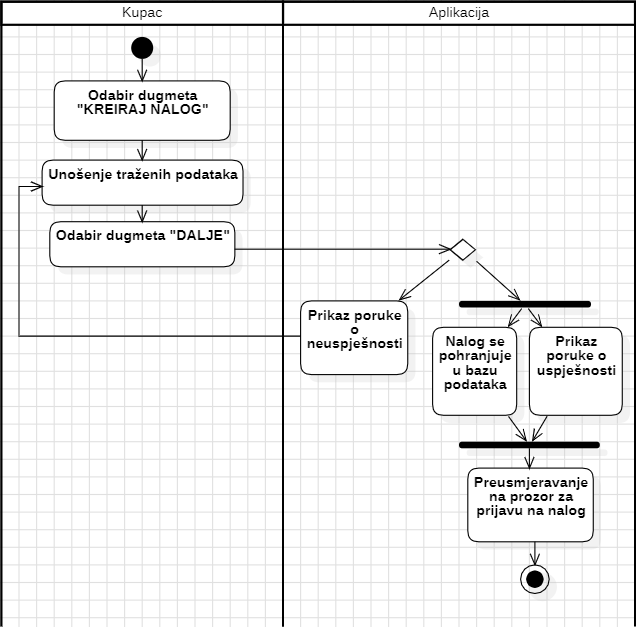
\includegraphics[width=14cm]{./img/14.png}
\end{center}

\pagebreak

\begin{center}
\begin{tabular}{|l|l|}
	\hline
	Oznaka: & F15 \\
	\hline
	Naziv: & PRIJAVA NA POTROŠAČKI NALOG \\
	\hline
	\smash{\raisebox{0ex}{Kratak opis:}}
	& Funkcionalnost koja kupcima omogućava\\
	& prijavu na svoj nalog \\
	\hline
	Učesnici: & Kupac \\
	\hline
	Preduslovi:
	& Kupac ima odgovarajući nalog. \\
	& Kupac ima potr. aplikaciju na svom računaru. \\
	\hline
	\smash{\raisebox{0ex}{Tok akcija:}}
	& 1. Kupac klikne na dugme "PRIJAVA NA\\
	& \hspace{10pt} NALOG" \\
	& 2. Kupac unosi korisničko ime i šifru \\
	& 3. Kupac klikne na dugme "DALJE" \\
	\hline
	\smash{\raisebox{0ex}{Postuslovi:}}
	& Kupac je preusmjeren na prozor koji mu omogućava \\
	& da pristupi funkionalnostima potrošačkog naloga \\ % TODO: Možda ovo i za restoranski nalog
	\hline
	\smash{\raisebox{0ex}{Alternativni tokovi i izuzeci:}}

	& 3.a. Uneseni podaci ne odgovaraju nekom nalogu \\
	& Postuslov: Kupac je obaviješten o neuspješnom\\
	& \hspace{50pt} pokušaju pristupa \\

	&\\

	& 3.b. Uneseni podaci nisu ispravni \\
	& Postuslov: Kupac je obaviješten o neuspješnom\\
	& \hspace{50pt} pokušaju pristupa \\

	\hline


\end{tabular}
\end{center}

\begin{center}
	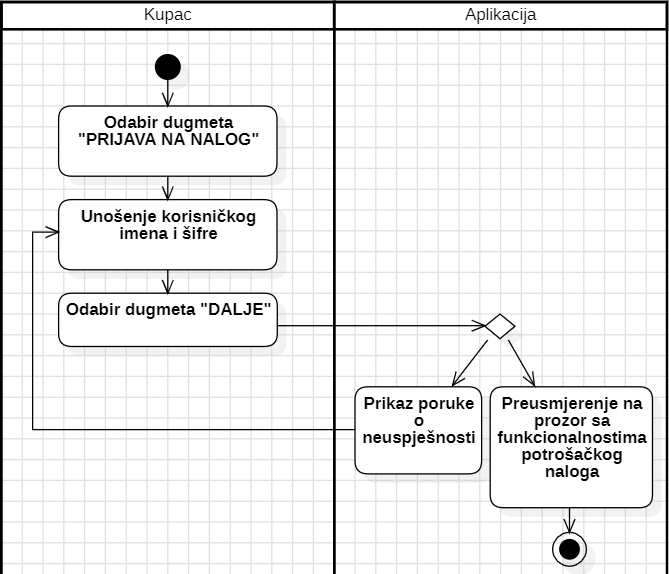
\includegraphics[width=14cm]{./img/15.png}
\end{center}

\pagebreak

\begin{center}
\begin{tabular}{|l|l|}
	\hline
	Oznaka: & F16 \\
	\hline
	Naziv: & PRETRAGA RESTORANA \\
	\hline
	\smash{\raisebox{0ex}{Kratak opis:}}
	& Funkcionalnost koja kupcima omogućava da pretraže\\
	& restorane koji su registrovani u softverskom sistemu, \\
	& te da odaberu iz kog restorana žele da naruče \\
	\hline
	Učesnici: & Kupac \\
	\hline
	Preduslovi:
	& Kupac ima odgovarajući nalog. \\
	& Kupac ima potr. aplikaciju na svom računaru. \\
	& Kupac je prijavljen na svoj nalog. \\
	\hline
	\smash{\raisebox{0ex}{Tok akcija:}}
	& 1. Kupac klikne na dugme "PRETRAŽI RESTORANE" \\
	& 2. Iz liste ponuđenih, kupac klikće na željeni restoran \\
	\hline
	\smash{\raisebox{0ex}{Postuslovi:}}
	& Kupac je preusmjeren na prozor za pregled restorana. \\
	\hline
	\smash{\raisebox{0ex}{Alternativni tokovi i izuzeci:}}

	&Nema.\\

	\hline

\end{tabular}
\end{center}

\begin{center}
	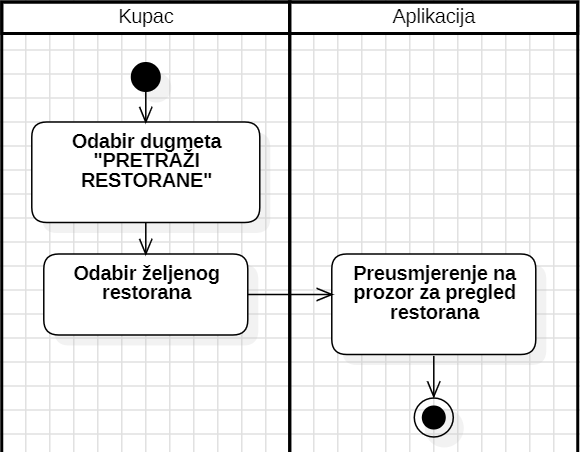
\includegraphics[width=14cm]{./img/16.png}
\end{center}

\pagebreak

% TODO: Narudžba

\begin{center}
\begin{tabular}{|l|l|}
	\hline
	Oznaka: & F17 \\
	\hline
	\smash{\raisebox{0ex}{Naziv:}}
	& PREGLED REST. NALOGA IZ PERSPEKTIVE\\
	& POTROŠAČA \\
	\hline
	\smash{\raisebox{0ex}{Kratak opis:}}
	& Funkcionalnost koja kupcima omogućava\\
	& pregled naloga restorana \\
	\hline
	Učesnici: & Kupac \\
	\hline
	Preduslovi:
	& Kupac ima odgovarajući nalog. \\
	& Kupac ima potr. aplikaciju na svom računaru. \\
	& Kupac je prijavljen na svoj nalog. \\
	\hline
	\smash{\raisebox{0ex}{Tok akcija:}}
	& 1. Kupac klikne na dugme "NARUČI IZ \\& \hspace{10pt} RESTORANA" \\
	\hline
	\smash{\raisebox{0ex}{Postuslovi:}}
	& Kupac je preusmjeren na prozor na kojem se \\
	& nalaze artikli iz restorana. \\
	\hline
	\smash{\raisebox{0ex}{Alternativni tokovi i izuzeci:}}

	&Nema.\\

	\hline

\end{tabular}
\end{center}

\begin{center}
	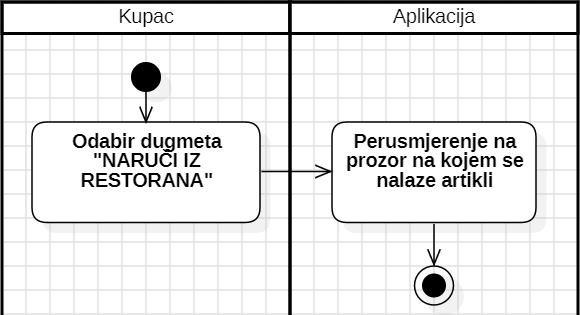
\includegraphics[width=14cm]{./img/17.png}
\end{center}

\pagebreak

\begin{center}
\begin{tabular}{|l|l|}
	\hline
	Oznaka: & F18 \\
	\hline
	Naziv: & PRAVLJENJE NARUDŽBE \\
	\hline
	\smash{\raisebox{0ex}{Kratak opis:}}
	& Funkcionalnost koja kupcima omogućava pregled \\
	& ponuda jednog restorana, pretragu i filtriranje \\
	& artikala istog, te pravljenje narudžbe \\
	\hline
	Učesnici: & Kupac \\
	\hline
	Preduslovi:
	& Kupac ima odgovarajući nalog. \\
	& Kupac ima potr. aplikaciju na svom računaru. \\
	& Kupac je prijavljen na svoj nalog. \\
	\hline
	\smash{\raisebox{0ex}{Tok akcija:}}
	& 1. Kupac klikne na dugme pored artikla koji \\
	& \hspace{10pt} želi da naruči. \\
	& 2. Kupac ponavlja korak 1 sve dok nije \\
	& \hspace{10pt} složio kompletnu narudžbu. \\
	& 3. Kupac klikne na dugme "NARUČI" \\
	& 4. Korisnik bira način plaćanja. \\
	\hline
	\smash{\raisebox{0ex}{Postuslovi:}}
	& Narudžba je dodana na red narudžbi restorana. \\
	& Kupac je obaviješten o uspješnosti podnošenja \\
	& narudžbe. Ukoliko je potrebno, dešava se i \\
	& novčana transakcija. Korisnik je preusmjeren \\
	& na \textit{glavni prozor}. \\
	\hline
	\smash{\raisebox{0ex}{Alternativni tokovi i izuzeci:}}

	& 1.a. Kupac piše u polje za pretraživanje \\
	& Postuslov: Ponuda artikala se sužava, tako \\
	& \hspace{50pt} da ostaju samo artikli koji sadrže \\
	& \hspace{50pt} riječi koje je korisnik unio. \\

	&\\

	& 1.b. Kupac klikne na jedan od ponuđenih filtera \\
	& Postuslov: Ponuda artikala se sužava, tako \\
	& \hspace{50pt} da ostaju samo artikli koji \\
	& \hspace{50pt} zadovoljavaju filter. \\

	&\\

	& 2.a. Kupac klikne na dugme "SKINI ARTIKL" \\
	& Postuslov: Artikl pored kojeg je dugme je skinut \\
	& \hspace{50pt} sa narudžbe. \\

	&\\

	& 3.a. Nije moguće napraviti narudžbu \\
	& Postuslov: Kupac je obaviješten o neuspješnosti \\
	& \hspace{51pt} pravljenja narudžbe. \\

	\hline

\end{tabular}
\end{center}

\begin{center}
	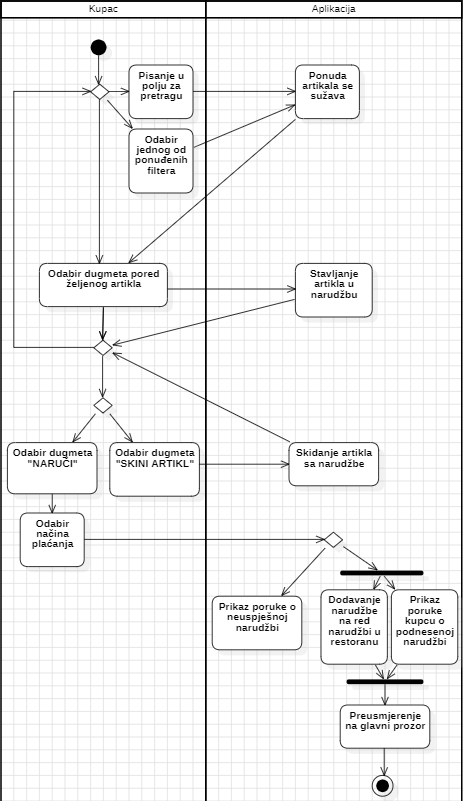
\includegraphics[width=14cm]{./img/18.png}
\end{center}

\pagebreak

\begin{center}
\begin{tabular}{|l|l|}
	\hline
	Oznaka: & F19 \\
	\hline
	Naziv: & AŽURIRANJE POTROŠAČKOG NALOGA \\
	\hline
	\smash{\raisebox{0ex}{Kratak opis:}}
	& Funkcionalnost koja kupcima omogućava\\
	& ažuriranje podataka na svom nalogu \\
	\hline
	Učesnici: & Kupac \\
	\hline
	Preduslovi:
	& Kupac ima odgovarajući nalog. \\
	& Kupac ima potr. aplikaciju na svom računaru. \\
	& Kupac je prijavljen na svoj nalog. \\
	\hline
	\smash{\raisebox{0ex}{Tok akcija:}}
	& 1. Kupac klikne na dugme "AŽURIRAJ NALOG" \\
	& 2. Kupac napravi željene izmjene \\
	& 3. Kupac klikne na dugme "POTVRDI" \\
	\hline
	\smash{\raisebox{0ex}{Postuslovi:}}
	& U bazi podataka se dešavaju tražene izmejene. \\
	& Kupac je vraćen na prethodni prozor. \\
	\hline
	\smash{\raisebox{0ex}{Alternativni tokovi i izuzeci:}}

	& 3.a. Uneseni podaci nisu ispravni \\
	& Postuslov: Kupac je obaviješten o neuspješnom \\
	& \hspace{51pt} pokušaju izmjene. \\
	\hline

\end{tabular}
\end{center}

\begin{center}
	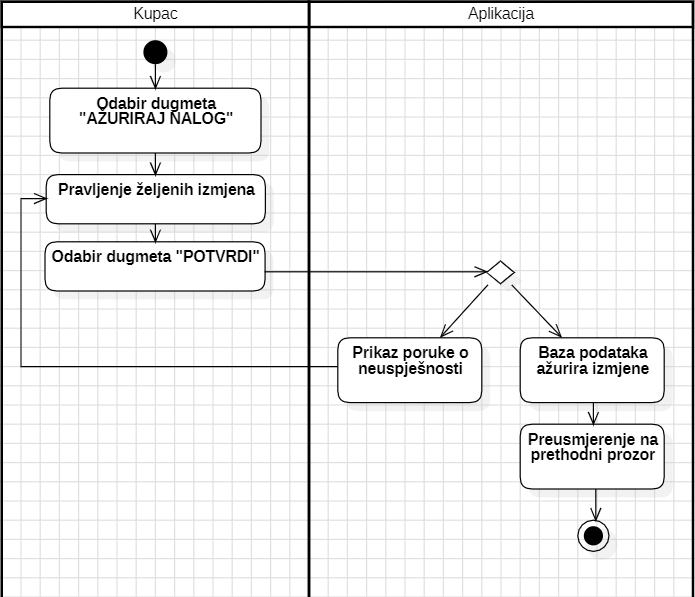
\includegraphics[width=14cm]{./img/19.png}
\end{center}

\pagebreak

\begin{center}
\begin{tabular}{|l|l|}
	\hline
	Oznaka: & F20 \\
	\hline
	Naziv: & PREGLED POTROŠAČKOG NALOGA \\
	\hline
	\smash{\raisebox{0ex}{Kratak opis:}}
	& Funkcionalnost koja kupcima omogućava\\
	& pregled svog naloga, kao i bivših narudžbi \\
	\hline
	Učesnici: & Kupac \\
	\hline
	Preduslovi:
	& Kupac ima odgovarajući nalog. \\
	& Kupac ima potr. aplikaciju na svom računaru. \\
	& Kupac je prijavljen na svoj nalog. \\
	\hline
	\smash{\raisebox{0ex}{Tok akcija:}}
	& 1. Kupac klikne na dugme "PREGLEDAJ\\
	& \hspace{10pt} BIVŠE NARUDŽBE" \\
	\hline
	\smash{\raisebox{0ex}{Postuslovi:}}
	& Kupac je preusmjeren na prozor na kojem\\
	& može da vidi svoje bivše narudžbe. \\
	\hline
	\smash{\raisebox{0ex}{Alternativni tokovi i izuzeci:}}

	&Nema.\\

	\hline

\end{tabular}
\end{center}

\begin{center}
	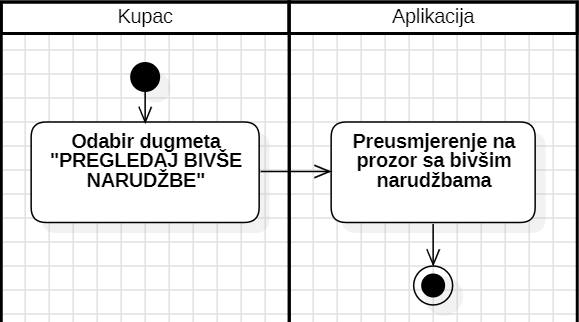
\includegraphics[width=14cm]{./img/20.png}
\end{center}

\pagebreak

\begin{center}
\begin{tabular}{|l|l|}
	\hline
	Oznaka: & F21 \\
	\hline
	Naziv: & PREGLED BIVŠIH NARUDŽBI \\
	\hline
	\smash{\raisebox{0ex}{Kratak opis:}}
	& Funkcionalnost koja kupcima omogućava\\
	& pregled narudžbi koje su pravili sa naloga koji \\
	& koriste \\
	\hline
	Učesnici: & Kupac \\
	\hline
	Preduslovi:
	& Kupac ima odgovarajući nalog. \\
	& Kupac ima potr. aplikaciju na svom računaru. \\
	& Kupac je prijavljen na svoj nalog. \\
	\hline
	\smash{\raisebox{0ex}{Tok akcija:}}
	& Nema. \\
	\hline
	\smash{\raisebox{0ex}{Postuslovi:}}
	& Nema. \\
	\hline
	\smash{\raisebox{0ex}{Alternativni tokovi i izuzeci:}}
	& Nema. \\
	\hline

\end{tabular}
\end{center}

\pagebreak

\begin{center}
\begin{tabular}{|l|l|}
	\hline
	Oznaka: & F22 \\
	\hline
	Naziv: & UKLANJANJE POTROŠAČKOG NALOGA \\
	\hline
	\smash{\raisebox{0ex}{Kratak opis:}}
	& Funkcionalnost koja kupcima omogućava \\
	& uklanjanje svog naloga iz baze podataka \\
	\hline
	Učesnici: & Kupac \\
	\hline
	Preduslovi:
	& Kupac ima odgovarajući nalog. \\
	& Kupac ima potr. aplikaciju na svom računaru. \\
	& Kupac je prijavljen na svoj nalog. \\
	\hline
	\smash{\raisebox{0ex}{Tok akcija:}}
	& 1. Kupac klikne na dugme "UKLONI NALOG" \\
	& 2. Kupac je preusmjeren na prozor na \\
	& \hspace{10pt} kojem se nalazi tekstualno polje na kojem \\
	& \hspace{10pt} piše "Da li ste sigurni da želite da uklonite\\
	& \hspace{10pt} svoj nalog?" i dugmad "DA" i "NE". \\
	& 3. Kupac klikne na "DA". \\
	\hline
	\smash{\raisebox{0ex}{Postuslovi:}}
	& Nalog se uklanja, i Kupac se vraća na \\
	& početni prozor potr. aplikacije. \\
	\hline
	\smash{\raisebox{0ex}{Alternativni tokovi i izuzeci:}}

	& 3.a. Kupac klikne na dugme "NE" \\
	& Postuslov: Kupac se vraća na prethodni \\
	& \hspace{50pt} prozor aplikacije. \\

	&\\

	& 3.b. Kupac klikne na dugme "DA", nije \\
	& \hspace{21pt} moguće ukloniti nalog \\
	& Postuslov: Kupac je obaviješten o neuspješnosti \\
	& \hspace{51pt} uklanjanja naloga. Kupac je vraćen \\
	& \hspace{51pt} na prethodni prozor. \\

	\hline

\end{tabular}
\end{center}

\begin{center}
	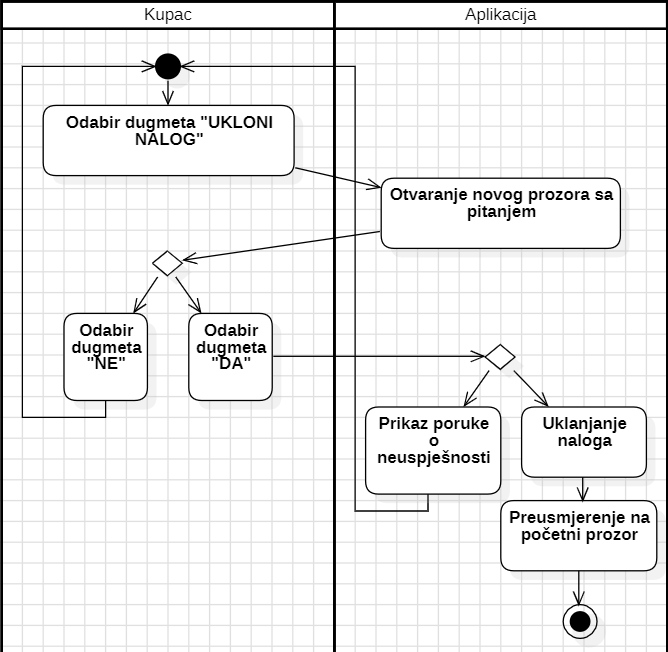
\includegraphics[width=14cm]{./img/22.png}
\end{center}

\pagebreak

\begin{center}
\begin{tabular}{|l|l|}
	\hline
	Oznaka: & F23 \\
	\hline
	Naziv: & ODJAVA SA NALOGA \\
	\hline
	\smash{\raisebox{0ex}{Kratak opis:}}
	& Funkcionalnost koja vlasniku, radniku ili kupcu \\
	& omogućava odjavu sa svog naloga \\
	\hline
	Učesnici: & Vlasnik, radnik ili kupac, ispod naveden kao korisnik \\
	\hline
	Preduslovi:
	& Korisnik ima odgovarajući nalog. \\
	& Korisnik ima odgovarajuću aplikaciju na svom računaru. \\
	& Korisnik je prijavljen na nalog. \\
	\hline
	\smash{\raisebox{0ex}{Tok akcija:}}
	& 1. Korisnik klikne na dugme "ODJAVI SE" \\
	\hline
	\smash{\raisebox{0ex}{Postuslovi:}}
	& Korisnik je preusmjeren na početni prozor \\& odgovarajuće aplikacije. \\
	\hline
	\smash{\raisebox{0ex}{Alternativni tokovi i izuzeci:}}
	& Nema. \\
	\hline

\end{tabular}
\end{center}

\begin{center}
	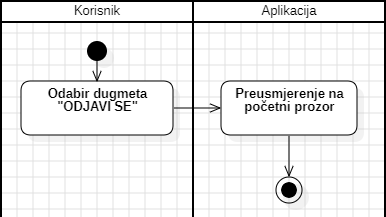
\includegraphics[width=14cm]{./img/23.png}
\end{center}

\pagebreak

\begin{center}
\begin{tabular}{|l|l|}
	\hline
	Oznaka: & F24 \\
	\hline
	Naziv: & ŠTAMPANJE RAČUNA \\
	\hline
	\smash{\raisebox{0ex}{Kratak opis:}}
	& Funkcionalnost koja vlasniku ili radniku \\
	& omogućava komunikaciju sa POS aparatom, u \\
	& cilju štampanja računa \\
	\hline
	Učesnici: & Vlasnik ili radnik, ispod naveden kao korisnik \\
	\hline
	Preduslovi:
	& Vlasnik ima odgovarajući nalog za svoj restoran. \\
	& Korisnik ima rest. aplikaciju na svom računaru. \\
	& Korisnik je prijavljen na nalog. \\
	\hline
	\smash{\raisebox{0ex}{Tok akcija:}}
	& 1. Korisnik klikne na dugme "ŠTAMPAJ RAČUN" \\
	\hline
	\smash{\raisebox{0ex}{Postuslovi:}}
	& Račun se štampa. \\
	\hline
	\smash{\raisebox{0ex}{Alternativni tokovi i izuzeci:}}
	& Nema. \\
	\hline

\end{tabular}
\end{center}

\begin{center}
	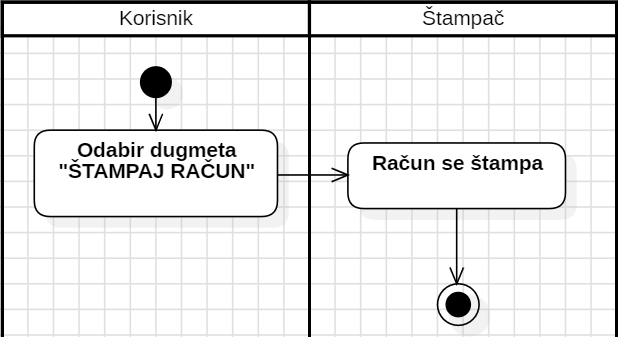
\includegraphics[width=14cm]{./img/24.png}
\end{center}

\pagebreak

\begin{center}
\begin{tabular}{|l|l|}
	\hline
	Oznaka: & F25 \\
	\hline
	Naziv: & POVRATAK NA PRETHODNI PROZOR \\
	\hline
	\smash{\raisebox{0ex}{Kratak opis:}}
	& Funkcionalnost koja korisniku omogućava \\
	& da se vrati na prethodni prozor aplikacije \\
	\hline
	Učesnici: & Vlasnik, radnik ili kupac, ispod naveden kao korisnik \\
	\hline
	Preduslovi:
	& Korisnik ima odgovarajući nalog. \\
	& Korisnik ima odgovarajuću aplikaciju na svom \\& računaru. \\
	& Korisnik je prijavljen na nalog. \\
	\hline
	\smash{\raisebox{0ex}{Tok akcija:}}
	& 1. Korisnik klikne na dugme "NAZAD" \\
	\hline
	\smash{\raisebox{0ex}{Postuslovi:}}
	& Korisnik je preusmjeren na prethodni prozor. \\
	\hline
	\smash{\raisebox{0ex}{Alternativni tokovi i izuzeci:}}
	& Nema. \\
	\hline

\end{tabular}
\end{center}

\begin{center}
	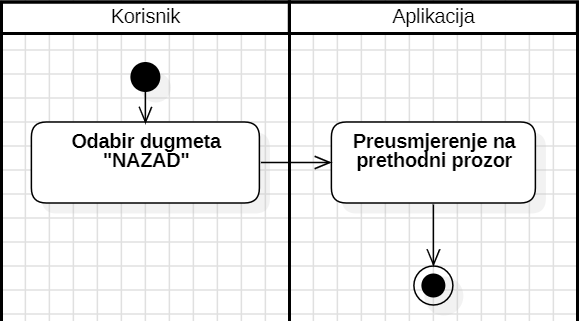
\includegraphics[width=14cm]{./img/25.png}
\end{center}

\pagebreak

\restoregeometry

\chapter{Rječnik}
Ispod ovog paragrafa je tabela termina koji su u dokumentu označeni
kosim tekstom, kao i njihova značenja.
\begin{center}
\begin{tabular}{|l|l|}
	\hline
	\textbf{Termin} & \textbf{Značenje} \\
	\hline
	\hline
	Kupac & Onaj koji kupuje brzu hranu \\\hline
	Vlasnik & Vlasnik datog restorana \\\hline
	Radnik & Radnik u datom restoranu, uključuje vlasnika \\\hline
	Resurs & Sastojci koji se koriste u pravljenju hrane u restoranu \\\hline
	Potrošačka aplikacija & \makecell[l]{Softverska aplikacija sistema FFDM namijenjena\\kupcima}\\\hline
	Restoranska aplikacija & \makecell[l]{Softverska aplikacija sistema FFDM namijenjena\\radnicima}\\\hline
	Glavni prozor & \makecell[l]{Prozor na koji je korisnik preusmjeren nakon prijave}\\\hline
	Početni prozor & \makecell[l]{Prozor koji se otvara na početku pokretanja jedne \\ od aplikacija}\\\hline
\end{tabular}
\end{center}

\chapter{Pregled korištenih skraćenica}

\begin{center}
\begin{tabular}{|l|l|}
	\hline
	\textbf{Skraćenica} & \textbf{Značenje} \\
	\hline
	\hline
	Potr. & Potrošački, potrošačka, potrošačko \\ \hline
	Rest. & Restoranski, restoranska, restoransko \\ \hline
\end{tabular}
\end{center}

% CPU, RAM, HDD, x86, x64

\end{document}
